%!TEX root = ../../common/main.tex

\section{Likelihood fit}
\label{sec:measurement_of_sin2beta:likelihood_fit}

This section presents the model developed to describe the data and estimate the
values and uncertainties of the physics observables using an \uEML fit. Starting
with a short review of the \uEML method, the \acp{PDF} in use to describe the
different dimensions and components are shown, and the fit model is outlined.

The \CP observables of interest \SJpsiKS and \CJpsiKS are estimated in a
multi-dimensional simultaneous \uEML fit. As summarised in
\cref{tab:measurement_of_sin2beta:data_preparation:observables} the seven
observables $\vect{x}$ are given by the reconstructed mass and decay time of the
\Bd candidate, its decay time error estimate, and its \OS and \SSpi tag decision
as well as the corresponding mistag estimates
%
\begin{equation}\label{eq:measurement_of_sin2beta:likelihood_fit:observables}
  \vect{x} = (\obsAllList)\eqpd  
\end{equation}
%
The extended likelihood for a total of $N = \sum_s N^s$ observed events in $s$
subsamples of data, where $n^s = \sum_j n_j^s$ are the expected candidate
numbers per subsample for the two categories $j = \{\Sig,\Bkg\}$, is then
defined as
%
\begin{equation}\label{eq:measurement_of_sin2beta:likelihood_fit:uEML}
  \Likelihood{}{}\left(\vect{\theta},\vect{n};\vect{x}\right) = \prod_{s}^{}\frac{\exponential{-n^s}}{N^s!} \prod_{i=1}^{N^s} \sum_{j}^{\{\Sig,\Bkg\}} n_{j}^{s} \Prob{j}{s} \left( \vect{x}_{i}^{s} ; \vect{\theta}_j \right )\eqcm
\end{equation}
%
where $\vect{n}$ is the vector of estimated candidate numbers, and
$\vect{\theta}$ the parameters with unknown values to be estimated by the \uEML
fit.

The software library \RooFit \cite{Verkerke:2003ir}---part of the \ROOT
\cite{Antcheva:2011zz} software framework---and its implementation of the
\Minuit algorithm is used to minimize the negative log-likelihood expression
$-\ln\Likelihood{}{}$.

In \cref{sec:measurement_of_sin2beta:likelihood_fit:pdfs} the \acp{PDF} used to
build the likelihood function are introduced shortly, before
\cref{sec:measurement_of_sin2beta:likelihood_fit:model} presents the complete
fit model employed by the \uEML fit. The approach to prevent any experimenter's
bias during the development of the fit model is described in
\cref{sec:measurement_of_sin2beta:likelihood_fit:blinding}. The results of the
fitter validation study are summarised in
\cref{sec:measurement_of_sin2beta:likelihood_fit:validation}.

% ------------------------------------------------------------------------------
\subsection{List of used \aclp{PDF}}
\label{sec:measurement_of_sin2beta:likelihood_fit:pdfs}

The following \acp{PDF} are employed to model the distributions of the fit
observables.

%...............................................................................
\subsubsection{Exponential}
\label{sec:measurement_of_sin2beta:likelihood_fit:pdfs:exponential}

The exponential function with the parameter $\alpha$ to describe \eg the
distribution of combinatorial background candidates with masses $m$
%
\begin{equation}\label{eq:measurement_of_sin2beta:likelihood_fit:pdfs:exponential}
  \ProbArg{\text{Exponential}}{}{m \given \alpha} \propto \exponential{\alpha m}\eqpd
\end{equation}

%...............................................................................
\subsubsection{Decay}
\label{sec:measurement_of_sin2beta:likelihood_fit:pdfs:decay}

The decay function is derived from the exponential function with $\alpha =
-\sfrac{1}{\tau}$, where $\tau$ describes the lifetime of candidates with decay
times $t$
%
\begin{equation}\label{eq:measurement_of_sin2beta:likelihood_fit:pdfs:decay}
  \ProbArg{\text{Decay}}{}{t \given \tau} \propto \exponential{- \frac{t}{\tau}}\eqpd
\end{equation}

%...............................................................................
\subsubsection{Gaussian}
\label{sec:measurement_of_sin2beta:likelihood_fit:pdfs:gaussian}

A simple Gaussian function described by the central value or mean $\mu$ and the
width $\sigma$ of the distribution
%
\begin{equation}\label{eq:measurement_of_sin2beta:likelihood_fit:pdfs:gaussian}
  \ProbArg{\text{Gaussian}}{}{x \given \mu, \sigma} \propto \frac{1}{\sigma\sqrt{2\pi}}\exponential{-\frac{1}{2} \left(\frac{x-\mu}{\sigma}\right)^2}\eqpd
\end{equation}

%...............................................................................
\subsubsection{Lognormal}
\label{sec:measurement_of_sin2beta:likelihood_fit:pdfs:lognormal}

The lognormal function is \eg used to describe the distribution of the decay
time error estimate $\obsTimeError$ and is parametrised by its median $\mu$ and
the parameter $k = \exponential{\sigma}$, where $\sigma$ is named the shape
parameter
%
\begin{equation}\label{eq:measurement_of_sin2beta:likelihood_fit:pdfs:lognormal}
  \ProbArg{\text{Lognormal}}{}{\obsTimeError \given \mu, k} \propto \frac{1}{\obsTimeError \sqrt{2\pi} \log (k)} \exponential{-\frac{\log^2 \left(\sfrac{\obsTimeError}{\mu}\right)}{2 \log^2(k)}}\eqpd
\end{equation}

%...............................................................................
\subsubsection{BDecay}
\label{sec:measurement_of_sin2beta:likelihood_fit:pdfs:bdecay}

A generalised exponential function to describe the time evolution of \Bmeson
states with decay times $t$. The coefficients $C$, $S$, and $D$ can be
adapted to describe \Bmeson mixing, \CP violation, and different asymmetries \eg
in the production of the \Bmesons. The \PDF is further parametrised by the
lifetime parameter $\tau$, the decay width difference $\DG$ and the mass
difference $\DM$ of the \Bmeson mass eigenstates.
%
\begin{multline}\label{eq:measurement_of_sin2beta:likelihood_fit:pdfs:bdecay}
  \ProbArg{\text{BDecay}}{}{\obsTime \given \dots} \propto \\ \exponential{- \frac{t}{\tau}}\left( \cosh (\DG t) + D \sinh (\DG t) + C \cos (\DM t) + S \sin (\DM t) \right)
\end{multline}

%...............................................................................
\subsubsection{Ipatia}
\label{sec:measurement_of_sin2beta:likelihood_fit:pdfs:ipatia}

The Ipatia \PDF \cite{Santos:2013gra} is a generalisation of the Crystal ball
\PDF \cite{set:crystalball}, marginalised over the a priori unknown per-event
mass resolution. The \PDF is used to describe the distribution of the
reconstructed $\B$ candidates mass $\obsMass$ and is parametrised as
%
\begin{multline}\label{eq:measurement_of_sin2beta:likelihood_fit:pdfs:ipatia}
  \ProbArg{\text{Ipatia}}{}{m \given \mu, \sigma, \lambda, \zeta, \beta, a_1, a_2, n_1, n_2} \propto \\
    \begin{cases}
      G(m, \mu, \sigma, \lambda, \zeta, \beta)    & \text{if $-a_1 < \frac{m-\mu}{\sigma} < a_2$} \\
      \frac{G(\mu - a_1 \sigma, \mu, \sigma, \lambda, \zeta, \beta)}{
        \left( 1 - \sfrac{m}{\left( n_1 \frac{G(\mu - a_1 \sigma, \mu, \sigma, \lambda, \zeta, \beta)}{G^\prime(\mu - a_1 \sigma, \mu, \sigma, \lambda, \zeta, \beta)} - a_1 \sigma \right)} \right)^{n_1}
      }     & \text{if $-a_1 > \frac{m-\mu}{\sigma}$} \\
      \frac{G(\mu - a_2 \sigma, \mu, \sigma, \lambda, \zeta, \beta)}{
        \left( 1 - \sfrac{m}{\left( n_2 \frac{G(\mu - a_2 \sigma, \mu, \sigma, \lambda, \zeta, \beta)}{G^\prime(\mu - a_2 \sigma, \mu, \sigma, \lambda, \zeta, \beta)} - a_2 \sigma \right)} \right)^{n_2}
      }     & \text{if $\phantom{-}a_2 < \frac{m-\mu}{\sigma}$} \\
  \end{cases}\eqcm
\end{multline}
%
where $G(x, \mu, \sigma, \lambda, \zeta, \beta)$ defines the generalised hyperbolic function
\begin{multline}\label{eq:measurement_of_sin2beta:likelihood_fit:pdfs:generalised_hyperbolic}
  G(x, \mu, \sigma, \lambda, \zeta, \beta) = \\
  \left(\left(x - \mu\right)^2 + A_\lambda^2(\zeta) \sigma^2 \right)^{\frac{1}{2} \lambda - \frac{1}{4}}
  \exponential{\beta (x - \mu)} K_{\lambda-\frac{1}{2}}
  \left(\zeta \sqrt{1 + \left(\sfrac{x - \mu}{A_\lambda(\zeta) \sigma}\right)^2} \right)\eqcm
\end{multline}
%
with the cylindrical harmonics $K_\lambda$ and
%
\begin{equation}
  A_\lambda^2(\zeta) = \frac{\zeta K_\lambda(\zeta)}{K_{\lambda+1}(\zeta)}\eqpd
\end{equation}
%
Here, $\mu$ and $\sigma$ are comparable to the mean and width known from a
Gaussian distribution. The parameters $\lambda$ and $\zeta$ describe the shape
of the central peak, $\beta$ characterises the skewness of the distribution.
The left and right side tails of the distribution are parametrised by $a_i$ and
$n_i$.

% ------------------------------------------------------------------------------
\subsection{Parametrisation of the fit model}
\label{sec:measurement_of_sin2beta:likelihood_fit:model}

The total \PDF is composed of two components for signal and background labelled
\enquote{$\Sig$} and \enquote{$\Bkg$}
%
\begin{equation}
  \Norm{\text{Total}}{}\Prob{\text{Total}}{} = \Norm{\Sig}{}\Prob{\Sig}{} + \Norm{\Bkg}{}\Prob{\Bkg}{}\eqcm
\end{equation}
%
where $\Norm{}{}$ are normalisation factors. As the mass and decay time are
uncorrelated the summed \PDF can be decomposed into a product of a mass and a
decay time \PDF. The decay time \PDF describes the conditional distributions of
the decay time and its dependent observable dimensions, the decay time
resolution estimate \obsTimeError, the flavour tags \obsTagOSSS, and their
associated mistag probability estimates \obsEtaOSSS.
%
\begin{multline}
  \ProbArg{\Sig/\Bkg}{}{\obsAllList} = \\ 
  \ProbArg{\Sig/\Bkg}{}{\obsMass} \cdot \ProbArg{\Sig/\Bkg}{}{\obsTime, \obsTimeError, \obsTagOS, \obsTagSS, \obsEtaOS, \obsEtaSS}
\end{multline}
%
As shown in \cref{sec:measurement_of_sin2beta:likelihood_fit:model:mistag} the
per-event mistag estimates are uncorrelated to the reconstructed decay time.
Hence, the signal decay time \PDF can be further decomposed into a product of
the conditional decay time \PDF $\ProbArg{\Sig}{}{\obsTime, \obsTagOS, \obsTagSS
\mid \obsTimeError, \obsEtaOS, \obsEtaSS}$ describing the \Bmeson time
evolution as well as the \CP violating effects, the \PDF
\ProbArg{\Sig}{}{\obsTimeError} describing the resolution estimate, and the
\acp{PDF} \ProbArg{\Sig}{}{\obsEtaOSSS} describing the mistag probability
estimates.
%
\begin{multline}
  \ProbArg{\Sig}{}{\obsTime, \obsTimeError, \obsTagOS, \obsTagSS, \obsEtaOS, \obsEtaSS} = \\ 
  \ProbArg{\Sig}{}{\obsTime, \obsTagOS, \obsTagSS \mid \obsTimeError, \obsEtaOS, \obsEtaSS} \cdot
  \ProbArg{\Sig}{}{\obsTimeError} \cdot
  \ProbArg{\Sig}{}{\obsEtaOS} \cdot
  \ProbArg{\Sig}{}{\obsEtaSS}
\end{multline}
%
As the background decay time \PDF does not depend on the mistag probability
distributions, only the decay time error estimate enters the conditional decay
time \PDF.
%
\begin{multline}
  \ProbArg{\Bkg}{}{\obsTime, \obsTimeError, \obsTagOS, \obsTagSS, \obsEtaOS, \obsEtaSS} = \\ 
  \ProbArg{\Bkg}{}{\obsTime, \obsTagOS, \obsTagSS \mid \obsTimeError} \cdot
  \ProbArg{\Bkg}{}{\obsTimeError} \cdot
  \ProbArg{\Bkg}{}{\obsEtaOS} \cdot
  \ProbArg{\Bkg}{}{\obsEtaSS}
\end{multline}
%
With this general structure being outlined, each single dimension and the
parametrisation of the signal and background components are explained. The
utilised \acp{PDF} are listed and it is explained which parameters are shared in
the categories of the simultaneous fit to the different data subsamples (\cf
\cref{sec:measurement_of_sin2beta:data_preparation:subsamples}).

%...............................................................................
\subsubsection{Mass}
\label{sec:measurement_of_sin2beta:likelihood_fit:model:mass}

The \textbf{signal} mass distribution is modelled using an Ipatia \PDF.
Individual parameters are chosen for the track types \catDD and \catLL. The
parameter $\zeta$ is always fixed to zero. The values of the tail parameters
$a_1, a_2, n_1, n_2$ and of the parameter $\lambda$ are determined on simulated
data and fixed to these values in the fit.

The \textbf{background} component is described by a single exponential \PDF. The
parameter $\alpha$ is shared among all subsamples except for \catDD and \catLL.

%...............................................................................
\subsubsection{Decay time}
\label{sec:measurement_of_sin2beta:likelihood_fit:model:decay_time}

The conditional \textbf{signal} decay time \PDF is given by
%
\begin{multline}
    \ProbArg{\Sig}{}{\obsTime, \obsTagOS, \obsTagSS \mid \obsTimeError, \obsEtaOS, \obsEtaSS} \\ 
  = \varepsilon_{\Sig}^{\text{\catAU,\catEB}}(\obsTimeTrue) \cdot \left(\ProbArg{\Sig}{}{\obsTime^\prime, \obsTagOS, \obsTagSS \mid \obsEtaOS, \obsEtaSS} \otimes \Resolution{\Sig}{}\left(\obsTime-\obsTimeTrue\right)\right)\eqcm
\end{multline}
%
where the acceptance function $\varepsilon_{\Sig}^{\text{\catAU,\catEB}}$ (\cf
\cref{sec:measurement_of_sin2beta:resolution_and_acceptance:acceptance:lower})
is implemented using cubic splines \cite{Karbach:2014qba} and the resolution
model $\Resolution{\Sig}{}\left(\obsTime-\obsTime^\prime\right)$ (\cf
\cref{sec:measurement_of_sin2beta:resolution_and_acceptance:resolution}) is
convolved with the \B physics \PDF.

In the following the \B physics \PDF is explained in detail. The theoretical
distributions---neglecting all experimental effects---for \Bd and \Bdbar mesons
($\ProbArg{\text{true}}{\Bd}{\obsTimeTrue}$ and
$\ProbArg{\text{true}}{\Bdbar}{\obsTimeTrue}$) are given by (\cf
\cref{eq:cpv_theory:flavour_physics:time_evolution:differential_decay_rates})
%
\begin{equation}
  \begin{split}
    \ProbArg{\text{true}}{\Bd}{\obsTimeTrue}    &= \frac{1}{\Norm{\obsTimeTrue}{\Bd}}    \exponential{-\sfrac{\obsTimeTrue}{\tau}} \left( 1 - S \sin(\DMd t) + C \cos (\DMd t) \right)\eqcm \\
    \ProbArg{\text{true}}{\Bdbar}{\obsTimeTrue} &= \frac{1}{\Norm{\obsTimeTrue}{\Bdbar}} \exponential{-\sfrac{\obsTimeTrue}{\tau}} \left( 1 + S \sin(\DMd t) - C \cos (\DMd t) \right)\eqcm
  \end{split}
\end{equation}
%
with normalisation factors
%
\begin{equation}
  \begin{split}
    \Norm{\obsTimeTrue}{\Bd}    &= \int_{t_\text{min}}^{t_\text{max}} \dif t \, \exponential{-\sfrac{\obsTimeTrue}{\tau}} \left( 1 - S \sin (\DMd t) + C \cos (\DMd t) \right)\eqspace\text{and} \\
    \Norm{\obsTimeTrue}{\Bdbar} &= \int_{t_\text{min}}^{t_\text{max}} \dif t \, \exponential{-\sfrac{\obsTimeTrue}{\tau}} \left( 1 + S \sin (\DMd t) - C \cos (\DMd t) \right)\eqpd
  \end{split}
\end{equation}
%
Here, $t_\text{min}$ and $t_\text{max}$ are the lower and upper limits of the
analysed decay time range (\cf
\cref{tab:measurement_of_sin2beta:data_preparation:observables}) and the parameter $\tau$ is the measured \Bd
lifetime. The conditional \acp{PDF} for true \Bd and \Bdbar mesons can now be
written as
%
\begin{equation}
  \begin{split}
    \ProbArg{\text{true}}{}{\obsTimeTrue\given\Bd}    &= \frac{\Norm{\obsTimeTrue}{\Bd}}{\Norm{\obsTimeTrue}{}}    \ProbArg{\text{true}}{\Bd}{\obsTimeTrue}\eqcm \\
    \ProbArg{\text{true}}{}{\obsTimeTrue\given\Bdbar} &= \frac{\Norm{\obsTimeTrue}{\Bdbar}}{\Norm{\obsTimeTrue}{}} \ProbArg{\text{true}}{\Bdbar}{\obsTimeTrue}\eqcm
  \end{split}
\end{equation}
%
with the normalisation factor
%
\begin{equation}
  \Norm{\obsTimeTrue}{} = \Norm{\obsTimeTrue}{\Bd} + \Norm{\obsTimeTrue}{\Bdbar}\eqpd
\end{equation}
%
A possible difference in the \Bd and \Bdbar production rates $R_{\B}$ and
$R_{\Bdbar}$ is treated by introducing the production asymmetry
%
\begin{equation}\label{eq:measurement_of_sin2beta:likelihood_fit:model:decay_time:production_asymmetry}
  A_P = \frac{R_{\Bdbar} - R_{\Bd}}{R_{\Bdbar} + R_{\Bd}}\eqcm
\end{equation}
%
leading to modified conditional \acp{PDF}
%
\begin{equation}\label{eq:measurement_of_sin2beta:likelihood_fit:model:decay_time:true_pdf}
  \begin{split}
    \ProbArg{\text{true}}{}{\obsTimeTrue\given\Bd}    &= \frac{\Norm{\obsTimeTrue}{\Bd}}{\Norm{\obsTimeTrue}{}}    (1 - A_P) \ProbArg{\text{true}}{\Bd}{\obsTimeTrue}     \eqspace \text{and} \\
    \ProbArg{\text{true}}{}{\obsTimeTrue\given\Bdbar} &= \frac{\Norm{\obsTimeTrue}{\Bdbar}}{\Norm{\obsTimeTrue}{}} (1 + A_P) \ProbArg{\text{true}}{\Bdbar}{\obsTimeTrue}  \eqpd
  \end{split}
\end{equation}
%
As the production flavour is unknown under experimental conditions the
measurement depends on the flavour tagging information of the \OS and \SSpi
tagging algorithms to decide whether the \Bmeson was produced as \Bd or \Bdbar.
With $\mistag_{i}$ is short for the calibrated mistag probability
$\mistag\left(\mistagestimate_{i}\right)$ the \PDF is then given as
%
\begin{equation}\label{eq:measurement_of_sin2beta:likelihood_fit:model:decay_time:measured_pdf_tagged_only}
\begin{split}
  \Prob{}{}(\obsTimeTrue, \obsTagOS, \obsTagSS &\mid \mistagOS, \mistagSS) = \\
        &\delta_{\obsTagOS,+1}\delta_{\obsTagSS,+1} \ProbArg{}{}{\obsTimeTrue \given +1, +1, \mistagOS, \mistagSS} \eqcm \\
      + &\delta_{\obsTagOS,+1}\delta_{\obsTagSS,-1} \ProbArg{}{}{\obsTimeTrue \given +1, -1, \mistagOS, \mistagSS} \eqcm \\
      + &\delta_{\obsTagOS,-1}\delta_{\obsTagSS,+1} \ProbArg{}{}{\obsTimeTrue \given -1, +1, \mistagOS, \mistagSS} \eqcm \\
      + &\delta_{\obsTagOS,-1}\delta_{\obsTagSS,-1} \ProbArg{}{}{\obsTimeTrue \given -1, -1, \mistagOS, \mistagSS} \eqcm 
  \end{split}
\end{equation}
%
with
%
\begingroup
  \thinmuskip=1mu
  \medmuskip=2mu plus 2mu minus 2mu
  \thickmuskip=3mu
\begin{equation}
  \begin{split}
    \Prob{}{}(\obsTimeTrue \mid +1, +1,\,& \mistagOS, \mistagSS ) = \\ 
      \Bigl(1 -& \mistagOS^{\Bd}\Bigr) \Bigl(1 - \mistagSS^{\Bdbar}\Bigr) \ProbArg{\text{true}}{}{\obsTimeTrue \given \Bd} \mistagOS^{\Bd} \mistagSS^{\Bdbar} \ProbArg{\text{true}}{}{\obsTimeTrue \given \Bdbar} \eqcm \\
    \Prob{}{}(\obsTimeTrue \mid +1, -1,\,& \mistagOS, \mistagSS ) = \\ 
      \Bigl(1 -& \mistagOS^{\Bd}\Bigr) \mistagSS^{\Bdbar} \ProbArg{\text{true}}{}{\obsTimeTrue \given \Bd} \mistagOS^{\Bd} \Bigl(1 - \mistagSS^{\Bdbar}\Bigr) \ProbArg{\text{true}}{}{\obsTimeTrue \given \Bdbar} \eqcm \\
    \Prob{}{}(\obsTimeTrue \mid -1, +1,\,& \mistagOS, \mistagSS ) = \\ 
      \mistagOS^{\Bd}& \Bigl(1 - \mistagSS^{\Bdbar}\Bigr) \ProbArg{\text{true}}{}{\obsTimeTrue \given \Bd} \Bigl(1 - \mistagOS^{\Bd}\Bigr) \mistagSS^{\Bdbar} \ProbArg{\text{true}}{}{\obsTimeTrue \given \Bdbar} \eqcm \eqthinspace \text{and} \\
    \Prob{}{}(\obsTimeTrue \mid -1, -1,\,& \mistagOS, \mistagSS ) = \\ 
      \mistagOS^{\Bd}& \mistagSS^{\Bdbar} \ProbArg{\text{true}}{}{\obsTimeTrue \given \Bd} \Bigl(1 - \mistagOS^{\Bd}\Bigr) \Bigl(1 - \mistagSS^{\Bdbar}\Bigr) \ProbArg{\text{true}}{}{\obsTimeTrue \given \Bdbar} \eqpd \\ 
  \end{split}
\end{equation}
\endgroup
%
\Cref{eq:measurement_of_sin2beta:likelihood_fit:model:decay_time:measured_pdf_tagged_only} 
only contains the \PDF to model decay time distributions of \B candidates where
tagging information from both tagging algorithms are available. If one of the
taggers does not provide an output, \ie the event falls into the
\catOS or \catSS category, the formulas can easily be adapted by setting
$\obsTagOSSS = \num{0}$ and/or $\mistagOSSS = \num{0.5}$. The expression
simplifies when explicitly implementing the \OS and \SSpi tag decisions
%
\begin{equation}\label{eq:measurement_of_sin2beta:likelihood_fit:model:decay_time:measured_pdf_tagged_only:simplified}
  \begin{split}
    \Prob{}{}(\obsTimeTrue &\mid \obsTagOS, \obsTagSS, \mistagOS, \mistagSS) = \\
      &\left( \frac{1 + \obsTagOS}{2} - \obsTagOS \mistagOS^{\Bd} \right)    \left( \frac{1 + \obsTagSS}{2} - \obsTagSS \mistagSS^{\Bd} \right) \ProbArg{\text{true}}{}{\obsTimeTrue \given \Bd}       \\
    + &\left( \frac{1 - \obsTagOS}{2} + \obsTagOS \mistagOS^{\Bdbar} \right) \left( \frac{1 - \obsTagSS}{2} - \obsTagSS \mistagSS^{\Bdbar} \right) \ProbArg{\text{true}}{}{\obsTimeTrue \given \Bdbar} \eqpd
  \end{split}
\end{equation}
%
Substituting $\ProbArg{\text{true}}{}{\obsTimeTrue \given \Bd}$ and
$\ProbArg{\text{true}}{}{\obsTimeTrue \given \Bdbar}$ making use of
\cref{eq:measurement_of_sin2beta:likelihood_fit:model:decay_time:true_pdf} and
making use of the definition of the tagging asymmetry $\deltamistag =
\mistag^{\Bd} - \mistag^{\Bdbar}$, 
\cref{eq:measurement_of_sin2beta:likelihood_fit:model:decay_time:measured_pdf_tagged_only:simplified} 
can be summarised as
%
\begingroup
  \thinmuskip=1mu
  \medmuskip=2mu plus 2mu minus 2mu
  \thickmuskip=3mu
\begin{multline}\raisetag{50pt}
  \ProbArg{}{}{\obsTimeTrue, \obsTagOS, \obsTagSS \given \obsEtaOS, \obsEtaSS} = \\
  \sum_{d^\prime} \Biggl[ \prod_{j} \zeta \left( d_j, \eta_j, d^{\prime} \right) \Biggr] \left( 1 - d^\prime A_P \right) \exponential{-\sfrac{\obsTimeTrue}{\tau}} \left\{ 1 - d^\prime \SJpsiKS \sin (\DMd \obsTimeTrue) + d^\prime \cos (\DMd \obsTimeTrue) \right\} \eqcm 
\end{multline}
\endgroup
%
with
%
\begin{equation}
  \zeta \left( d_j, \eta_j, d^{\prime} \right) = 1 + d_j \left( 1 - 2 \left[ \mistag(\mistagestimate_j) + d^{\prime} \frac{\Delta\mistag(\mistagestimate_j)}{2} \right] \right) \eqcm
\end{equation}
%
where the calibration of the mistag estimates is implied by
$\mistag(\mistagestimate)$ and $\Delta\mistag(\mistagestimate)$ and $d^\prime$
takes the value $+1$ ($-1)$ for the $\Bd$ ($\Bdbar$) signal component.

The \textbf{background} decay time distribution is modelled using sums of
exponential decay functions. Three decay \acp{PDF} are used to describe the
distributions in the \catLL and the (\catDD and \catOS) subsamples. The sum of
two decay \acp{PDF} is used to parametrise the \PDF describing the (\catDD and
(\catSS or \catBS)) subsamples. The \PDF parameters including the
pseudo-lifetimes are shared among all categories except for \catDD and \catLL.
In the \catDD subsample also individual parameters are chosen depending on the
tagging category. 

The applied resolution model is the same as for the signal component.

%...............................................................................
\subsubsection{Decay time error estimate}
\label{sec:measurement_of_sin2beta:likelihood_fit:model:decay_time_error}

For most subsamples the \textbf{signal} component's distribution is parametrised
using two lognormal \acp{PDF}. The lognormal \acp{PDF} in the (\catLL and
\catOS) subsample share a common median parameter. For candidates lying in the
(\catLL and (\catSS or \catBS)) subsamples a single lognormal \PDF is sufficient
to describe the decay time error estimate distribution. Individual parameters
are chosen depending on the track type and tagging categories, and in case of
the (\catDD and \catOS) category, also on the trigger category.

The \textbf{background} \PDF is composed of two lognormal distributions. In the
\catLL subsample individual parameters are chosen depending on the track type
and tagging categories. Candidates lying in the (\catDD and \catOS and \catAU)
subsample only share parameters in the \catOO and \catOT categories. In all
other subsamples the parameters are shared except for the track type category.

The parameter values are determined in a multi-dimensional fit to the mass,
decay time, and decay time error estimate distributions and subsequently fixed
in the nominal fit to reduce fit times.

%...............................................................................
\subsubsection{Mistag estimate}
\label{sec:measurement_of_sin2beta:likelihood_fit:model:mistag}

The complicated shapes of the mistag estimate distributions have to be modelled
empirically. Popular approaches to model non-parametric distributions are \eg
Gaussian kernel estimations and splines \cite{Karbach:2014qba}. The later one is
used here. Splines are piece-wise defined polynomials parametrised by interval
boundaries (\emph{knots}), values at these knots, and boundary conditions to
ensure a continuous and smooth function. To model the mistag estimate
distributions cubic splines are used as base splines.

For $n$ knots, there are $n+2$ base splines, and accordingly $n+2$ fit
parameters modelling the shape of the resulting \PDF. The knot positions are
chosen arbitrarily at points of noticeable changes in the shape of the described
distributions.

The used knots for the \obsEtaOS and \obsEtaSS distributions are
%
\begin{equation*}
\begin{split}
  \text{\acs{OS} knots} &= \{0.06, 0.10, 0.14, 0.165, 0.23, 0.3, 0.34, 0.36, 0.42, 0.44, 0.48\} , \\
  \text{\acs{SSpi} knots} &= \{0.16, 0.26, 0.36, 0.41, 0.46, 0.482279\} .
\end{split}
\end{equation*}
%
The explanation for the exceptional value of the last \SSpi knot can be found in
the pre-calibration applied. Originally, the \SSpi mistag estimates are cut at
values above $\num{0.44}$. The pre-calibration then shifts this boundary towards
the given value (\cref{sec:flavour_tagging:calibration:ss}). Likewise,
\OS candidates with a mistag estimate larger than $\num{0.48}$ are considered as
\OS untagged. This choice was made to speed up the fit time and to ensure fit
stability. As the candidates removed by this cut hold large mistags, the
reduction of the effective tagging efficiency is found to be insignificant.

The spline parameters for \textbf{signal} and \textbf{background} are determined
in a multi-dimensional fit including mass, decay time, and mistag estimate and
are fixed later on, to achieve a better fit performance. Both, the \OS and the
\SSpi mistag distributions are fitted using cubic splines with different spline
parameters for \catDD and \catLL and otherwise sharing them through all
categories. Only in the signal \OS distributions the differences depending on
the track type are negligible so the parameters are shared in the \catDD and
\catLL categories.

\paragraph{Correlation between \OS and SS\pionbfsf mistag estimates}

To check if the two dimensions of $\obsEtaOS$ and $\obsEtaSS$ factorise, the
linear Pearson correlation coefficient $\rho$ is calculated on the \sweighted
nominal data set. To clarify the significance of the values the bootstrap method
(\ie \enquote{random sampling with replacement}, \cf \eg \cite{Behnke:2013pga})
is used to get \SI{95}{\percent} \CL intervals for the correlation
coefficients. 
\Cref{tab:measurement_of_sin2beta:likelihood_fit:model:mistag:os_ss_correlations} 
lists the calculated linear correlation coefficients separately for \catDD and
\catLL as well as combined while always distinguishing between signal and
background. Overall the linear correlations are small, so the factorisation is
valid.
%
\begin{table}
\centering
\caption{Correlations and their \SI{95}{\percent} \acp{CL} between \OS and
\SSpi mistag estimates.}
\label{tab:measurement_of_sin2beta:likelihood_fit:model:mistag:os_ss_correlations}
\begin{tabular}{
  l
  S[table-number-alignment = left, table-text-alignment = center]
  r@{,\,}l
  S[table-number-alignment = left, table-text-alignment = center]
  r@{,\,}l
}
\toprule
            & \multicolumn{3}{c}{Signal}                                                            & \multicolumn{3}{c}{Background} \\
            & {$\rho_\text{\obsEtaOS,\obsEtaSS}$} & \multicolumn{2}{c}{\SI{95}{\percent} \acs*{CL}} & {$\rho_\text{\obsEtaOS,\obsEtaSS}$} & \multicolumn{2}{c}{\SI{95}{\percent} \acs*{CL}} \\
\midrule
\catDD      & 0.0731            & ($0.0306$ & $0.1155$)  &  0.0555           & ($0.0139$  & $0.0972$) \\
\catLL      & 0.0854            & ($0.0270$ & $0.1454$)  & -0.0465           & ($-0.219$  & $0.136$)  \\
combined    & 0.077             & ($0.041$  & $0.112$)   &  0.0507           & ($0.0101$  & $0.0919$) \\
\bottomrule
\end{tabular}
\end{table}

\paragraph{Correlation between decay time and \OS/SS\pionbfsf mistag estimates}

The same ansatz as before is chosen to test the correlation between the decay
time distributions and the mistag estimates.
\Cref{tab:measurement_of_sin2beta:likelihood_fit:model:mistag:mistag_time_correlations} 
shows no significant correlations between the decay time and the \OS/\SSpi
mistag estimates.
%
\begin{table}
\centering
\caption{Correlations and their \SI{95}{\percent} \acp{CL} between the mistag
estimates $\eta_\text{\acs{OS}/\acs{SSpi}}$ and the reconstructed \Bd decay
time.}
\label{tab:measurement_of_sin2beta:likelihood_fit:model:mistag:mistag_time_correlations}
\begin{tabular}{
  l
  S[table-alignment = center, table-column-width = 1.5cm]
  r@{,\,}l
  S[table-alignment = center, table-column-width = 1.5cm]
  r@{,\,}l
}
\toprule
           & \multicolumn{3}{c}{Signal}                                          & \multicolumn{3}{c}{Background} \\
           & {$\rho_{\eta,t}$} & \multicolumn{2}{c}{\SI{95}{\percent} \acs*{CL}} & {$\rho_{\eta,t}$} & \multicolumn{2}{c}{\SI{95}{\percent} \acs*{CL}} \\
\midrule
\OS        & -0.0046 & ($-0.0375$ & $0.0272$) & -0.0601 & ($-0.1086$ & $-0.0135$) \\
\SSpi      &  0.0223 & ($-0.0104$ & $0.0535$) & -0.002  & ($-0.048$  & $ 0.044$)  \\
\bottomrule
\end{tabular}
\end{table}

% ------------------------------------------------------------------------------
\subsection{Experimenter's bias}
\label{sec:measurement_of_sin2beta:likelihood_fit:blinding}

To minimise a potential experimenter's bias, a blinding transformation is
applied to the \CP observables $\SJpsiKS$ and $\CJpsiKS$ by adding an obfuscated
offset to the fit parameters. This does not affect the uncertainty estimates and
still allows to compare and reproduce the fit outcome. The offset is drawn from
a uniform distribution using a random number generator. The random seed is
generated using a so called blinding string. To ensure a sufficient ambiguity
the range of the uniform distribution is chosen to be ${[-2,2]}$. The blinding
string applied to conceal the estimated value of $\SJpsiKS$ is
\texttt{SJpsiKS2011und2012} and for $\CJpsiKS$ it is chosen to be
\texttt{CJpsiKS2011und2012}.

% ------------------------------------------------------------------------------
\subsection{Fitter validation}
\label{sec:measurement_of_sin2beta:likelihood_fit:validation}

The likelihood model described before and its code implementation is validated
using \ToyMC simulated and regular \MC simulated data.

%...............................................................................
\subsubsection{\Aclp{ToyMC}}
\label{sec:measurement_of_sin2beta:likelihood_fit:validation:toy_mc}

An external \ToyMC generator \cite{wishahi:2015bhf} is employed to scrutinise
the \PDF used in the fit. It generates distributions for the dimensions mass,
decay time, decay time error estimate, and mistag estimate, correctly models
the per-event tag and mistag for two tagging algorithms, comprises tagging and
production asymmetries, as well as tagged background events. Making use of the
signal to background ratios found on data a simulated data set is generated and
fitted afterwards. No significant deviations from the generated values are
found.

In addition the nominal \PDF is used to sample distributions. The subsequent fit
to the simulated data allows to check if the fit's parameter values and
uncertainties estimates are unbiased. In the generation the \CP parameters are
unblinded and set to $\SJpsiKS = \num{0.7}$ and $\CJpsiKS = \num{0.03}$. All
other parameters are set to the values estimated on data using the nominal fit
model. The results from $\num{1000}$ iterations of generating an fitting are
shown in \cref{fig:measurement_of_sin2beta:likelihood_fit:validation:toy_mc}. No
bias is observable.
%
\begin{figure}[ht]
\centering
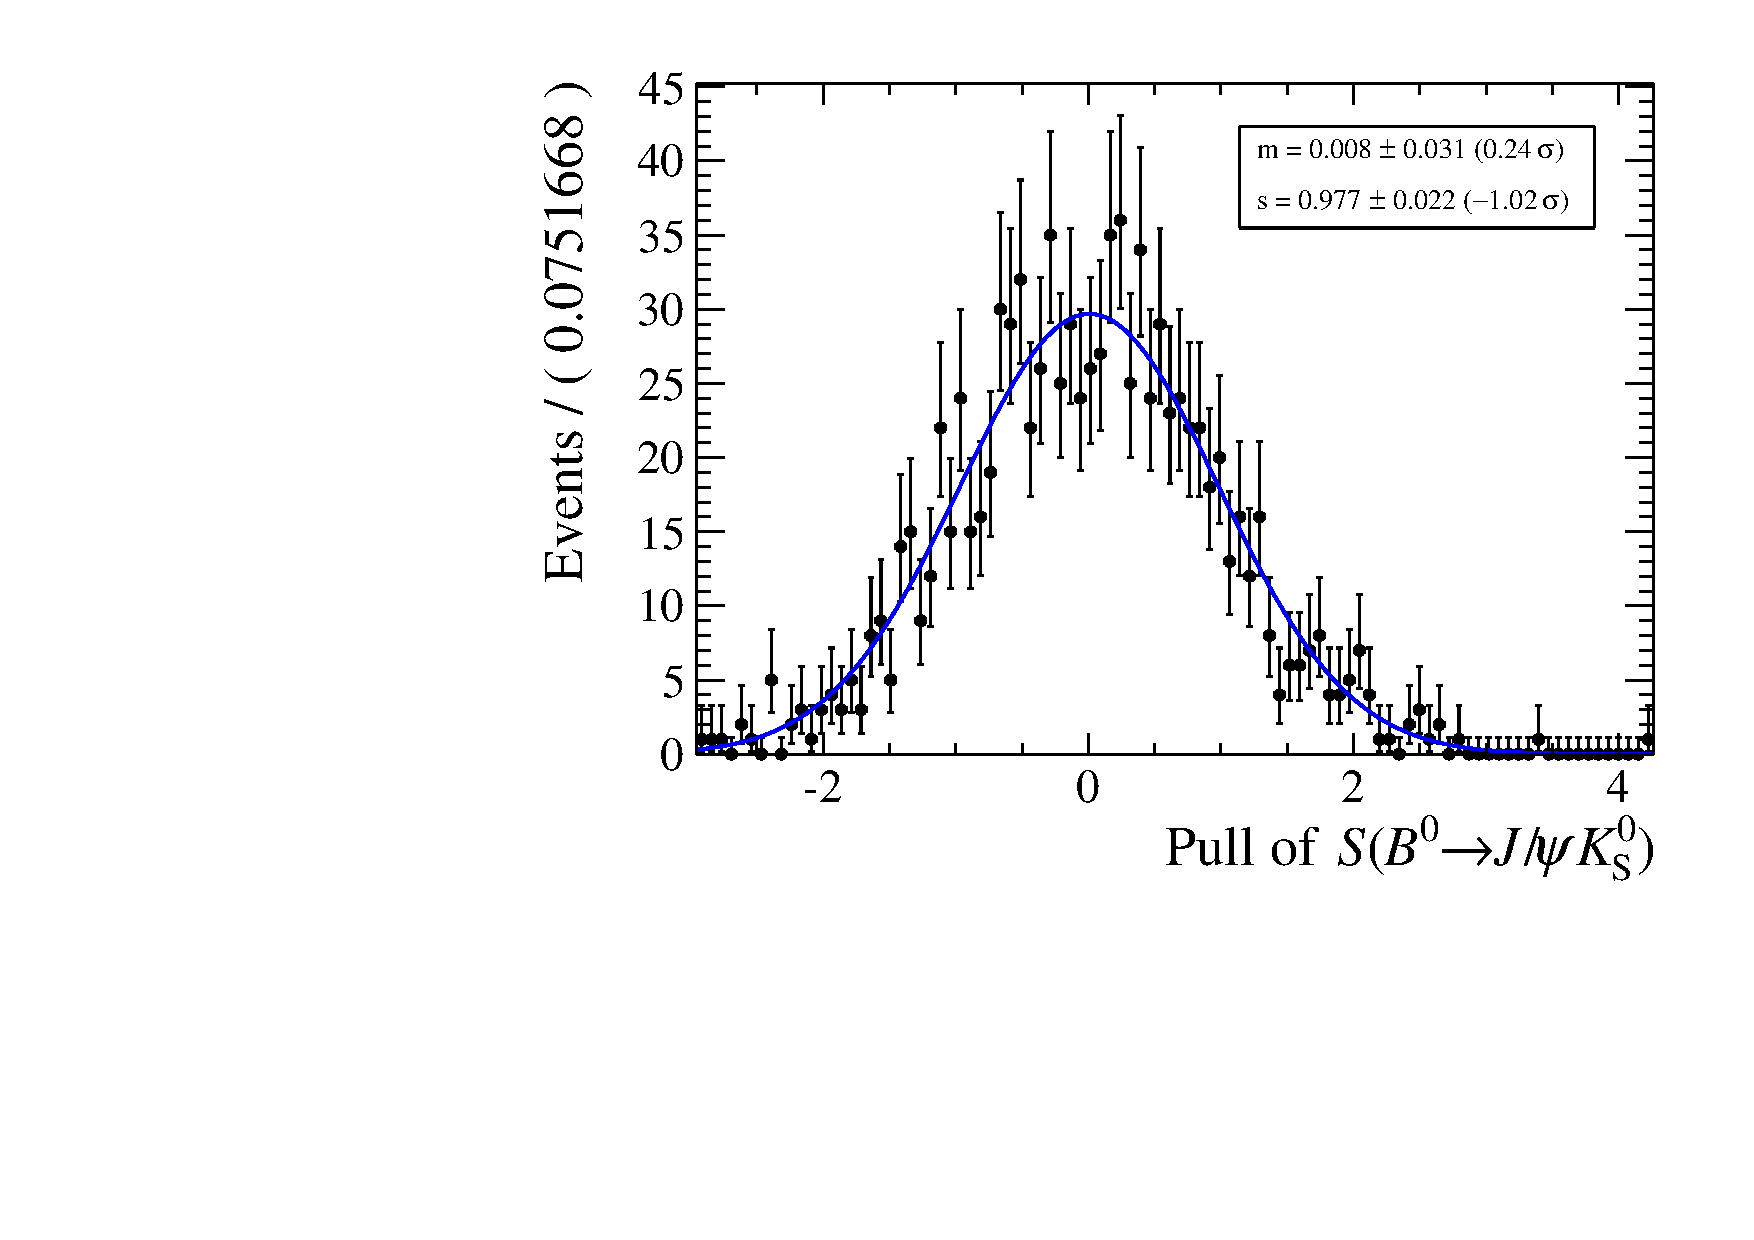
\includegraphics[width=0.48\textwidth]{private/content/measurement-of-sin2beta/figs/toy_fitter_validation_s_pull.pdf}
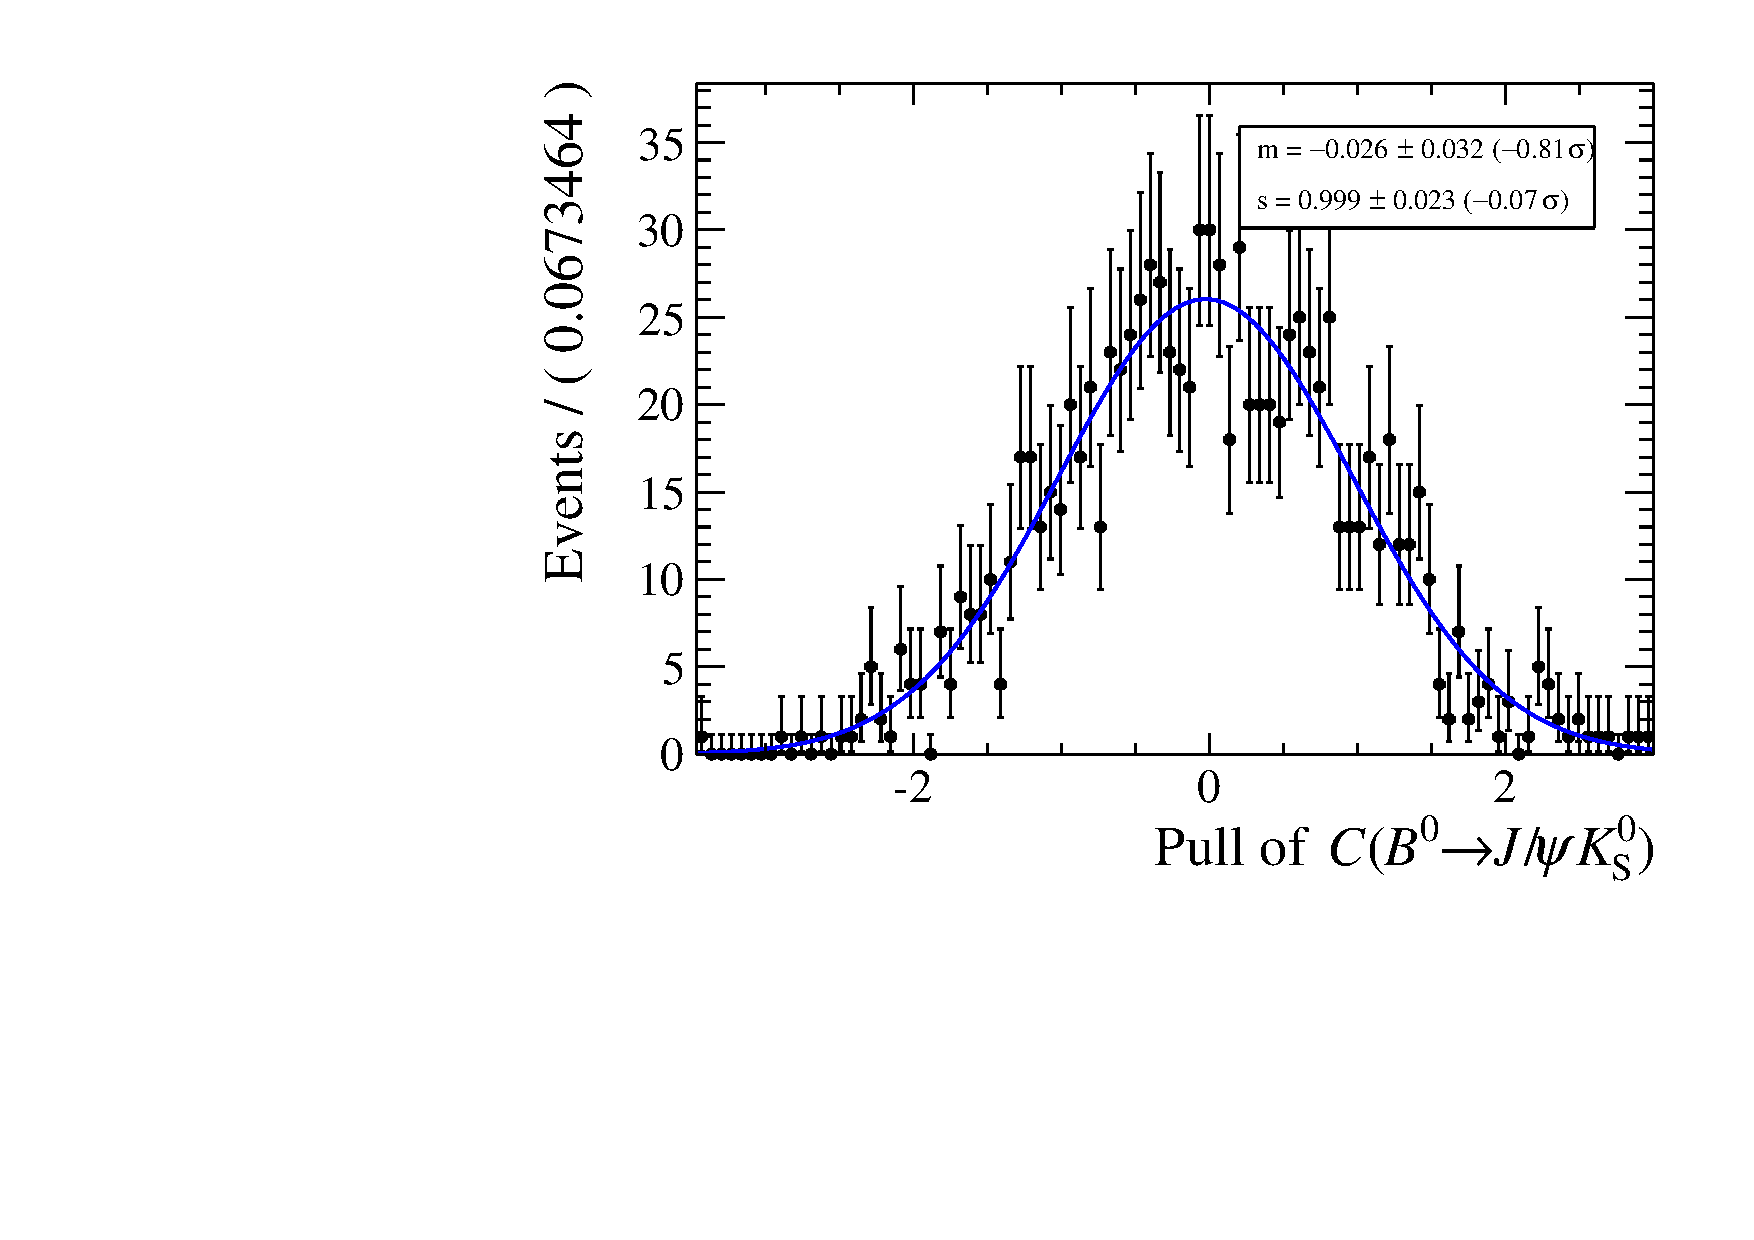
\includegraphics[width=0.48\textwidth]{private/content/measurement-of-sin2beta/figs/toy_fitter_validation_c_pull.pdf}     \\
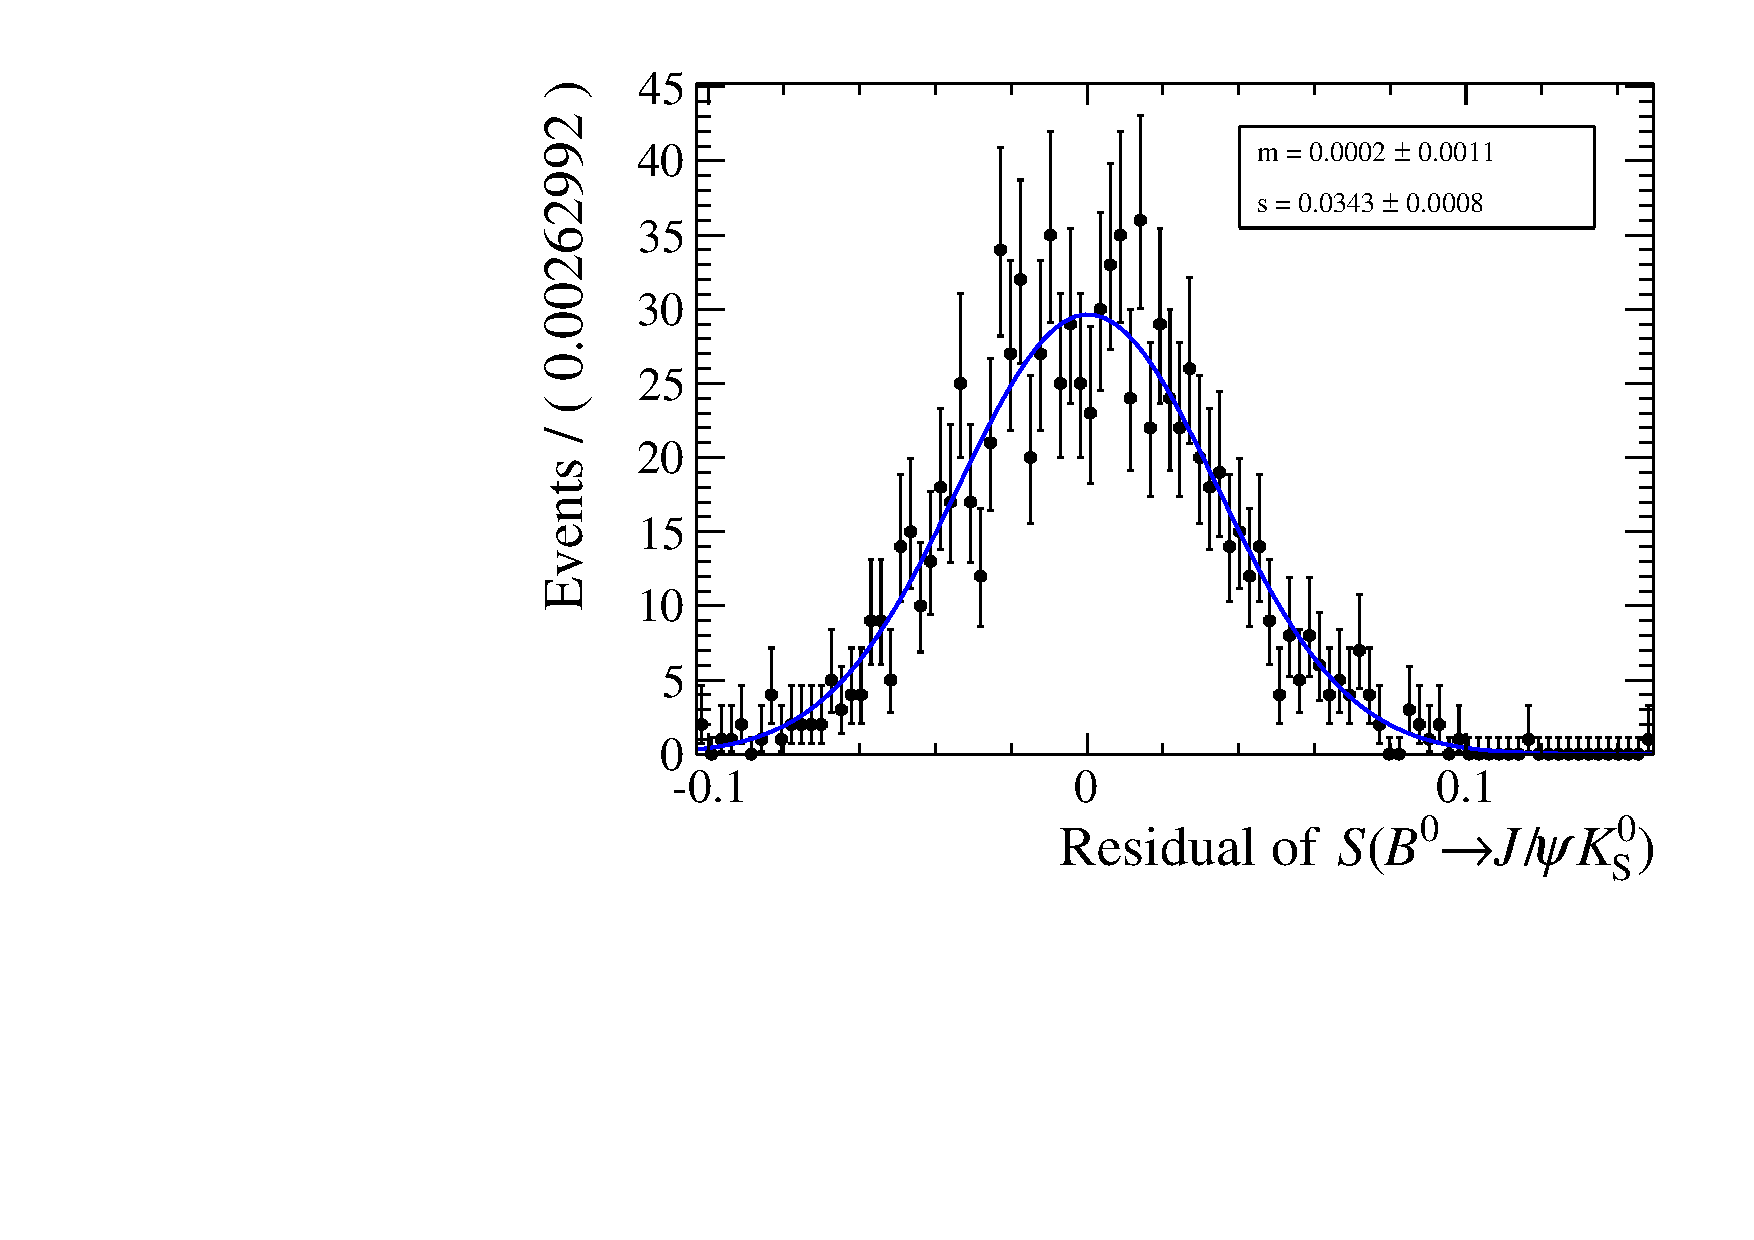
\includegraphics[width=0.48\textwidth]{private/content/measurement-of-sin2beta/figs/toy_fitter_validation_s_res.pdf}
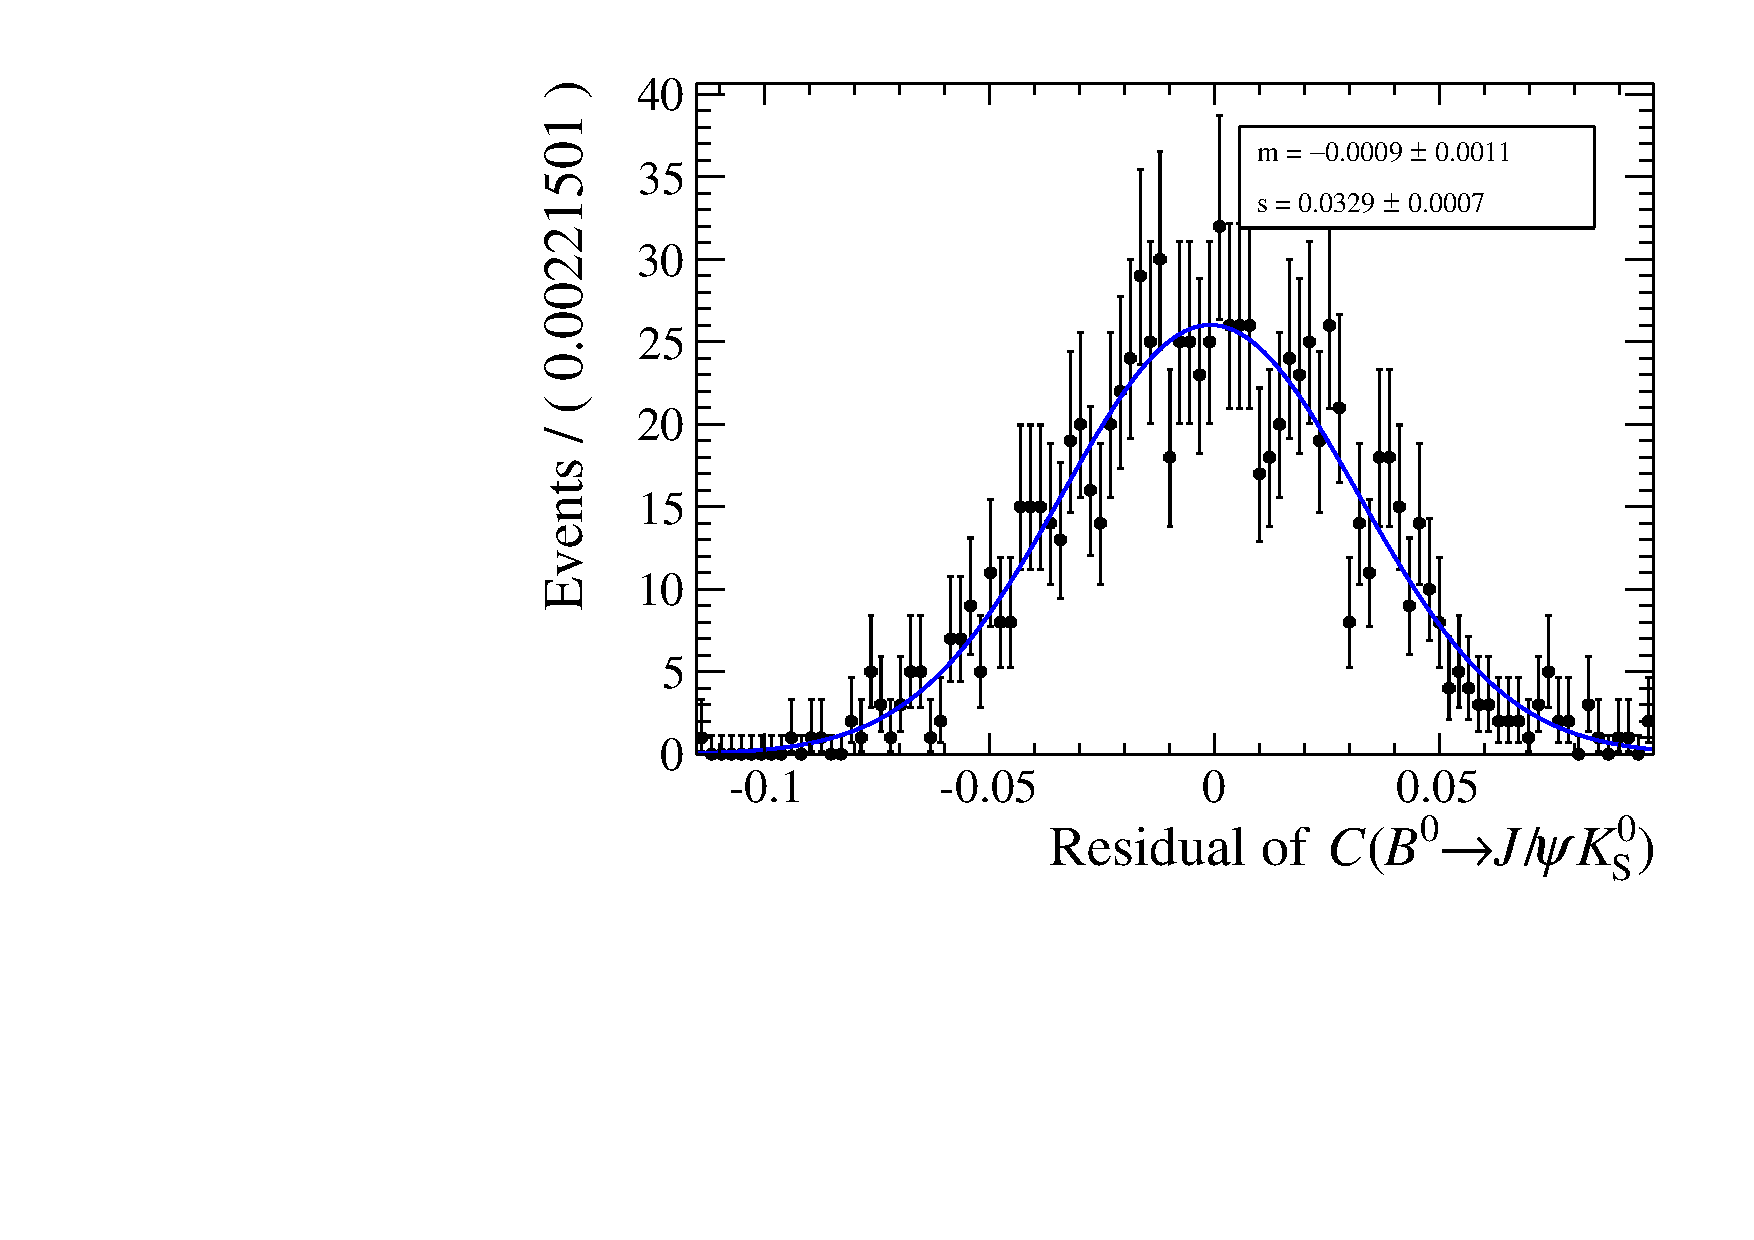
\includegraphics[width=0.48\textwidth]{private/content/measurement-of-sin2beta/figs/toy_fitter_validation_c_res.pdf}
\caption{Pull (top) and residual (bottom) distributions of \SJpsiKS (left) and
\CJpsiKS (right) in the fitter validation using \ac{ToyMC}.}
\label{fig:measurement_of_sin2beta:likelihood_fit:validation:toy_mc}
\end{figure}

%...............................................................................
\subsubsection{Signal \acs*{MC}}
\label{sec:measurement_of_sin2beta:likelihood_fit:validation:signal_mc}

To further validate the nominal fit model, a fit on signal \MC
(\cref{sec:measurement_of_sin2beta:data_preparation:datasamples:mc}) is
performed and the fit results are compared to the generation values of
$\SJpsiKS^{\text{Gen}} = \num{0.699716075}$, $\CJpsiKS^{\text{Gen}} = \num{0}$,
and $\tau_{\Bd}^{\text{Gen}} = \SI{1.519068}{\pico\second}$ (see
\cref{tab:measurement_of_sin2beta:data_preparation:datasamples:mc:decfile}).
\Cref{eq:measurement_of_sin2beta:likelihood_fit:validation:signal_mc} presents
the results. Both \CP parameters, as well as the \Bd lifetime are perfectly
compatible with the generation values.
%
\begin{equation}\label{eq:measurement_of_sin2beta:likelihood_fit:validation:signal_mc}
\begin{split}
  \SJpsiKS^{\text{SigMC}}   &= \num[separate-uncertainty=true]{0.714 \pm 0.032} \eqcm \\
  \CJpsiKS^{\text{SigMC}}   &= \num[separate-uncertainty=true]{0.012 \pm 0.028} \eqcm \\
  \tau_{\Bz}^{\text{SigMC}} &= \SI[separate-uncertainty=true]{1.521  \pm 0.009}{\pico\second} \eqpd \\
\end{split}
\end{equation}

%...............................................................................
\subsubsection{Cocktail \acs*{MC}}
\label{sec:measurement_of_sin2beta:likelihood_fit:validation:cocktail_mc}

Further, the fit model is tested on a simulated data set containing both signal
and background. For this study, the signal \MC sample is enriched with background
events generated from the background \PDF of the nominal fit model according to
the signal to background ratio observed in data. The fit results are shown in
\cref{eq:measurement_of_sin2beta:likelihood_fit:validation:cocktail_mc}. Again
all measured parameters are perfectly compatible with the generation values.
%
\begin{equation}\label{eq:measurement_of_sin2beta:likelihood_fit:validation:cocktail_mc}
\begin{split}
  \SJpsiKS^{\text{CocktailMC}}   &= \num[separate-uncertainty=true]{0.722 \pm 0.029}  \eqcm \\
  \CJpsiKS^{\text{CocktailMC}}   &= \num[separate-uncertainty=true]{0.008 \pm 0.027}  \eqcm \\
  \tau_{\Bz}^{\text{CocktailMC}} &= \SI[separate-uncertainty=true]{1.506  \pm 0.010}{\pico\second} \eqpd \\
\end{split}
\end{equation}
